\documentclass[12pt]{report}
\usepackage{hyperref}
\usepackage[pdftex]{graphicx}
\usepackage[normalem]{ulem}
\usepackage[utf8]{inputenc}
\usepackage[english,frenchb,francais]{babel}
\usepackage[T1]{fontenc}
\usepackage{hyperref}
\usepackage{geometry}
\usepackage{wrapfig}
\geometry{hmargin=1.5cm,vmargin=1.5cm}

\begin{document}
  \begin{titlepage}
    \centering
        \vfill
        {\rule{\linewidth}{.5pt}
        \huge
            Optimisation par algorithme génétique\\
          \large
            Influence du paramétrage\\
          \rule{\linewidth}{.5pt}
            \vskip2cm
            Swan Launay - Gabriel Vaubaillon\\
        }
        \vfill
        
\includegraphics[height=1.7cm]{logo/polytech.jpg}
        \hfill
        
\includegraphics[height=1.7cm]{logo/usmb.png}
  \end{titlepage}
  \pagenumbering{Roman}
  \chapter{Préambule}
    \section{Remerciements}
      Ce rapport représente l'aboutissement d'un projet de 40 heures qui s'est déroulé entre octobre 2018 et avril 2019. Nous tenons tout d'abord à remercier Gilles Fraisse pour son soutien, sa pédagogie, mais aussi pour le temps qu'il a passé à nous accompagner.

      Nous tenons aussi à remercier l'Université Savoie Mont Blanc (USMB) pour la mise à disposition des documents nécessaires à la réalisation de ce projet par le biais, notamment, de la bibliothèque universitaire.

      Nous remercions enfin Polytech Annecy - Chambéry pour nous avoir permis d'effectuer ce projet sur notre temps de travail universitaire et plus globalement pour nous avoir proposé un travail de ce type.

    \section{Résumé}
      L'optimisation par algorithme génétique permet d'obtenir de bonnes approximations de résolutions pour différents problèmes (avec un ou plusieurs objectifs). De façon générale, les algorithmes génétiques sont construits de telle façon à ce que l'on puisse faire varier certains paramètres. C'est ces mêmes paramètres qui vont déterminer la qualité et la fiabilité du résultat, mais aussi qui vont faire varier de façon plus ou moins significative le temps de résolution. Il s'agit alors de trouver un juste milieu entre le temps résolution et la fiabilité du résultat.

  \chapter{Introduction}
    Selon la \emph{Théorie de l'évolution} \cite{darwin} de Charles Darwin, l'évolution des espèces est issue de mutations aléatoires qui surviennent lors de la conception d'une nouvelle génération d'individus. Si cette mutation permet à l'individus d'être plus adapté à son milieu de vie, alors il aura plus de chance d'atteindre l'age adulte et d'engendrer une nouvelle génération.
    Les algorithmes génétiques sont une application directe du darwinisme à l'informatique.\\
    De nos jours, ces algorithmes permettent de résoudre des problèmes d'optimisation, c'est à dire de maximiser ou de minimiser numériquement une ou plusieurs fonctions.
    La branche des mathématiques qu'est l'optimisation est un élément central dans le monde de l'ingéniérie ou on cherche dans de très nombreux cas à minismier plusieurs problèmes à la fois et à obtenir un solution de qualité dans un laps de temps court.\\
    Ce rapport présente deux types d'algorithme génétique différents, le premier est adapaté à une optmisation mono-objectif (un seul problème), alors que l'autre l'est pour des problèmes multiobjectifs. Pour chacun des deux algorithmes nous détaillerons à la fois le principe de résolution, mais aussi l'influence du paramétrage.

  \tableofcontents
  \chapter{Quelques définitions}
    objectif :
    individus :
    solution optimale :
    Pareto :
    Paretor de référence :
    extremum local :



  \chapter{Optimisation à objectif unique}
    \pagenumbering{arabic}
    \section{Algorithme}
      \subsection{Principe}
        \begin{wrapfigure}{r}{6cm}
          \centering
          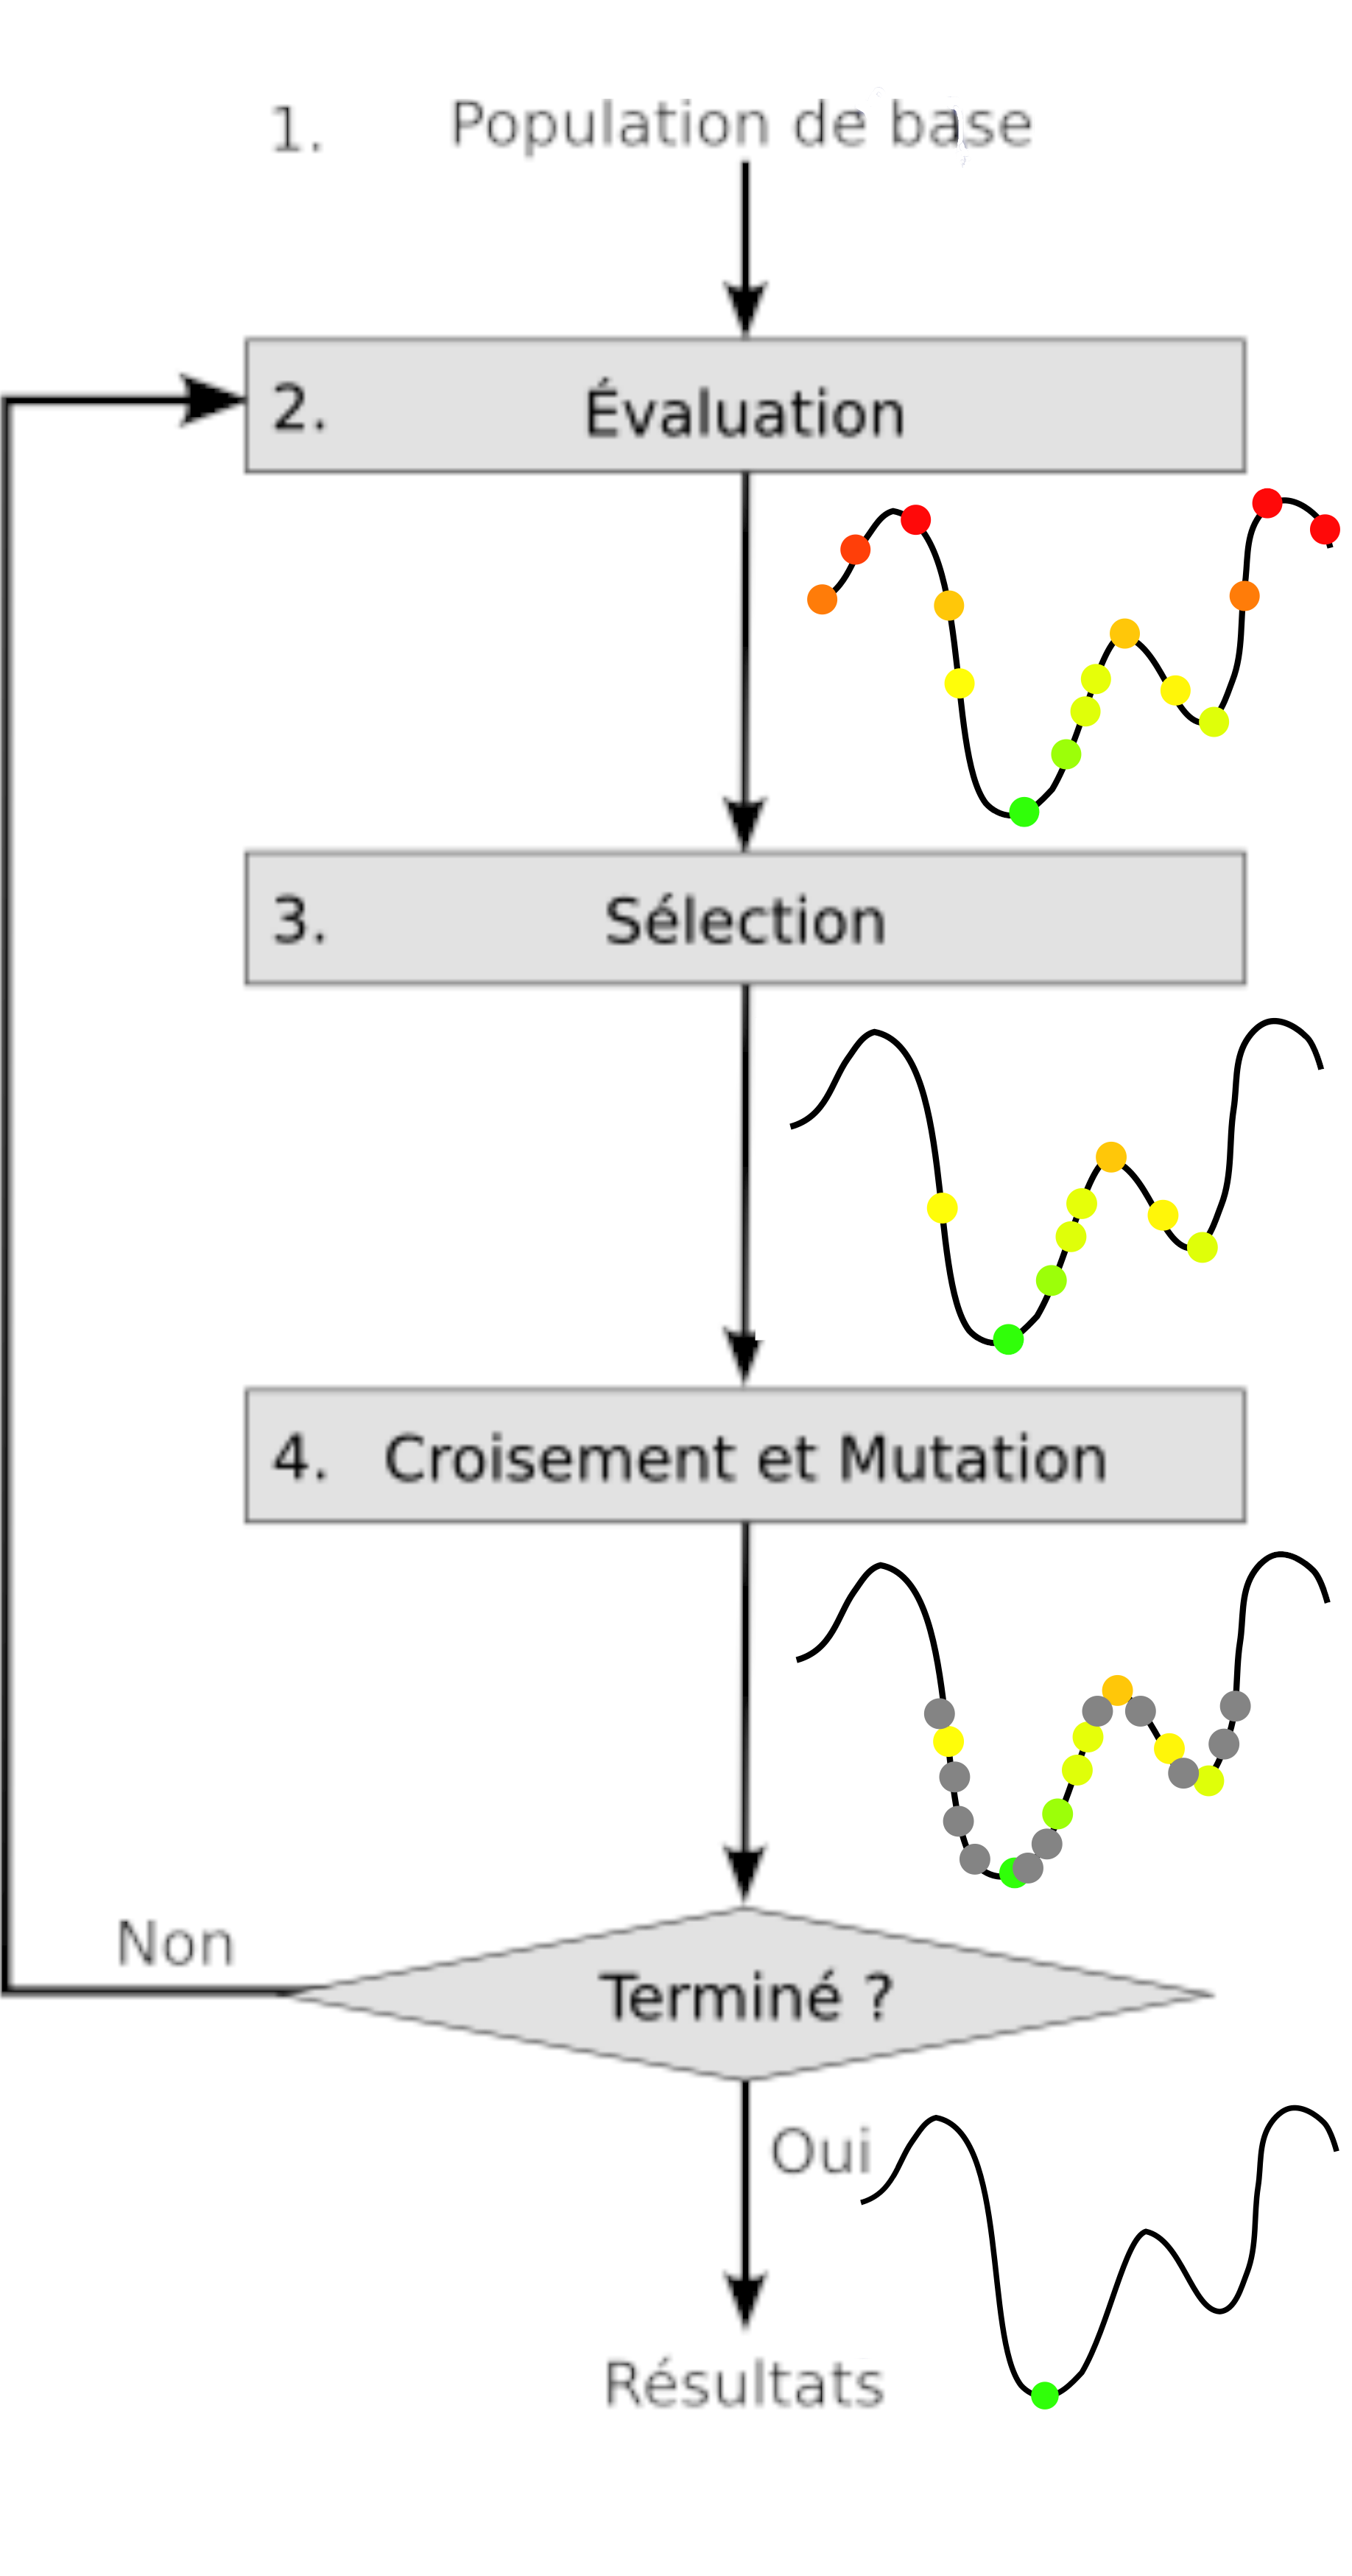
\includegraphics[width=5cm]{img/schema_algo_single.png}
          \caption{Fonctionnement}
        \end{wrapfigure}
        Hormis quelques variations dans leur conception, les algorithmes génétiques ont pratiquement tous le même principe de fonctionnement.
        Le logigramme ci-joint illustre le fonctionnement de base d'un algorithme mono-objectif.
        On commence par génèrer de façon aléatoire une population de base qui servira d'initialisation de notre algorithme.
        Chaque individus de cette population est alors évalué, on lui attribut une valeur qui va déterminer sa position par rapport à la solution optimale recherchée (ici le minimum de la fonction).
        Une selection est ensuite effectuée en gardant les meilleurs résultats, mais aussi en gardant un certain pourcentage de valeurs considérées comme de moyenne/faible qualité. Cette dernière opération permet entre-autre à l'algorithme de ne pas tomber dans un extremum local.
        A partir de cette séléction, l'algorithme va procéder à deux étapes :
        \begin{enumerate}
          \item Le croisement (Crossover) :
          il consiste à partager (croiser) les particulartiés de deux individus parents pour engendrer une nouvelle population d'individus conservant ces mêmes particularités. A noter qu'il existe plusieurs méthodes de croisement (linéaire, à n points, ... etc) qui ont chacunes leur particularités. Dans notre cas c'est le croisement à 3 points de rotation qui est utilisé, son fonctionnement est expliqué par la figure \ref{sch_crossover}.
          \emph{Remarque : On retrouve cette opération en biologie sous le nom de "brassage génétique" qui illustre le principe d'héridité de la théorie de Darwin \cite{darwin}.}
          \begin{figure}[h]
            \centering
            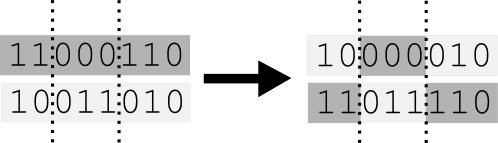
\includegraphics{img/crossover.png}
            \caption{Analogie binaire d'un croisement à 3 points de rotation}
            \label{sch_crossover}
          \end{figure}
          \item La mutation :
          contrairement au croisement qui conserve les particularités des individus au cours des générations, la mutation altère certains individus de manière aléatoire. Cette oprération complète l'opération de séléction précédement évoquée afin d'éviter de tomber dans un extremum local.
          \emph{Remqarque : cette opération illutsre le Principe de variation de la théorie de Darwin en biologie \cite{darwin}.}
        \end{enumerate}

    \section{Optimisation unidimensionnelle / multidimensionnelle}.
      \begin{wrapfigure}{r}{7cm}
        \centering
        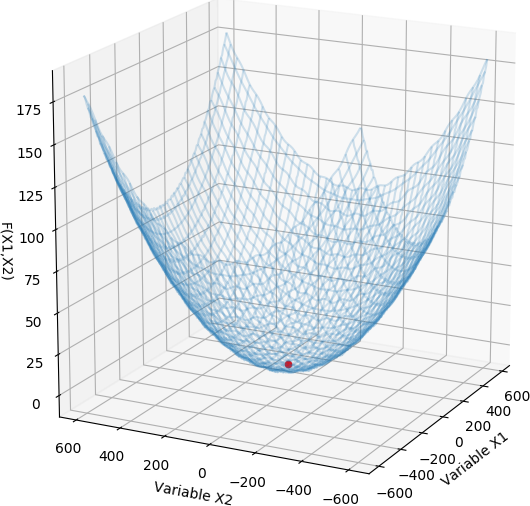
\includegraphics[width=6cm]{img/3,2.png}
        \caption{Fonction Griwank \cite{wiki5} en bleu, solution de l'algorithme en rouge}
        \label{ex_r2}
      \end{wrapfigure}
      Bien que l'obtimisation mono-objectif signifie l'optimisation d'un seul problème, ce problème peut tout de même comporter plusieurs variable, on parle alors d'optimisation multidimensionnelle ($\mathbb{R}^n \rightarrow \mathbb{R}$). Il est possible de représenter graphiquement de tels problèmes jusqu'à une dimension égale à 2 (Voir figure \ref{ex_r2}).

    \section{Influence du paramétrage }
      Lors de sont exécution, un algorithme génétique est soumis à un paramétrage préalablement défini par l'utilisateur. Ce paramétrage va agir sur le comportement et sur la capacité de l'algorithme à trouver des solutions de qualité. Dans le cadre de ce projet, c'est  l'influence de ce paramétrage qui nous intéresse, on chercher donc à faire varier les paramètres pour se rendre compte de l'influence qu'ils ont sur l'algorithme.

      \subsection{Protocole}
        \begin{wrapfigure}{r}{7cm}
          \centering
          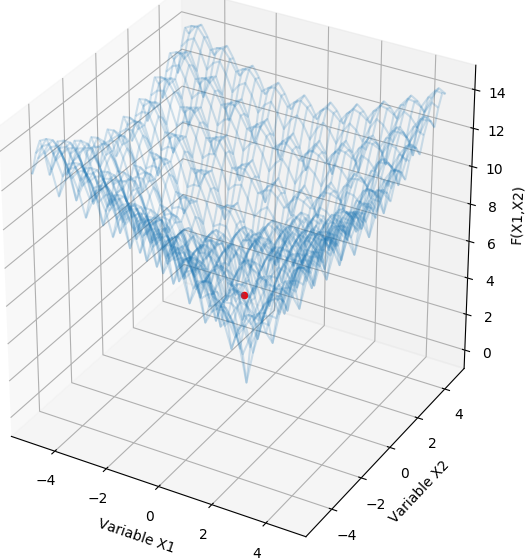
\includegraphics[width=6cm]{img/ackley.png}
          \caption{Fonction Ackley \cite{wiki5}}
          \label{ackley}
        \end{wrapfigure}
        \begin{itemize}
          \item Dans cette partie la fonction dont on cherche le minimum se nommme Ackley et est définie tel que :
          $$
          \left\{
            \begin{array}{ll}
               \forall x,y \in [-5,5], f(x,y) = -20 * e^{-0.2\sqrt{0.5(x^2+y^2)}} $$ \\
               Solution : f(0,0) = 0 $$
            \end{array}
          \right.
          $$
          \item Un programme informatique a été réalisé pour faire varier ces paramètre automatiquement.
        \end{itemize}

      \subsection{Taille de la population}
        L'exécution du programme pour la variation de la taille de la population retourne les graphiques des figures \ref{evo_pop_size_brut} et \ref{evo_pop_size_moy}.

        \begin{figure}[h]
          \centering
          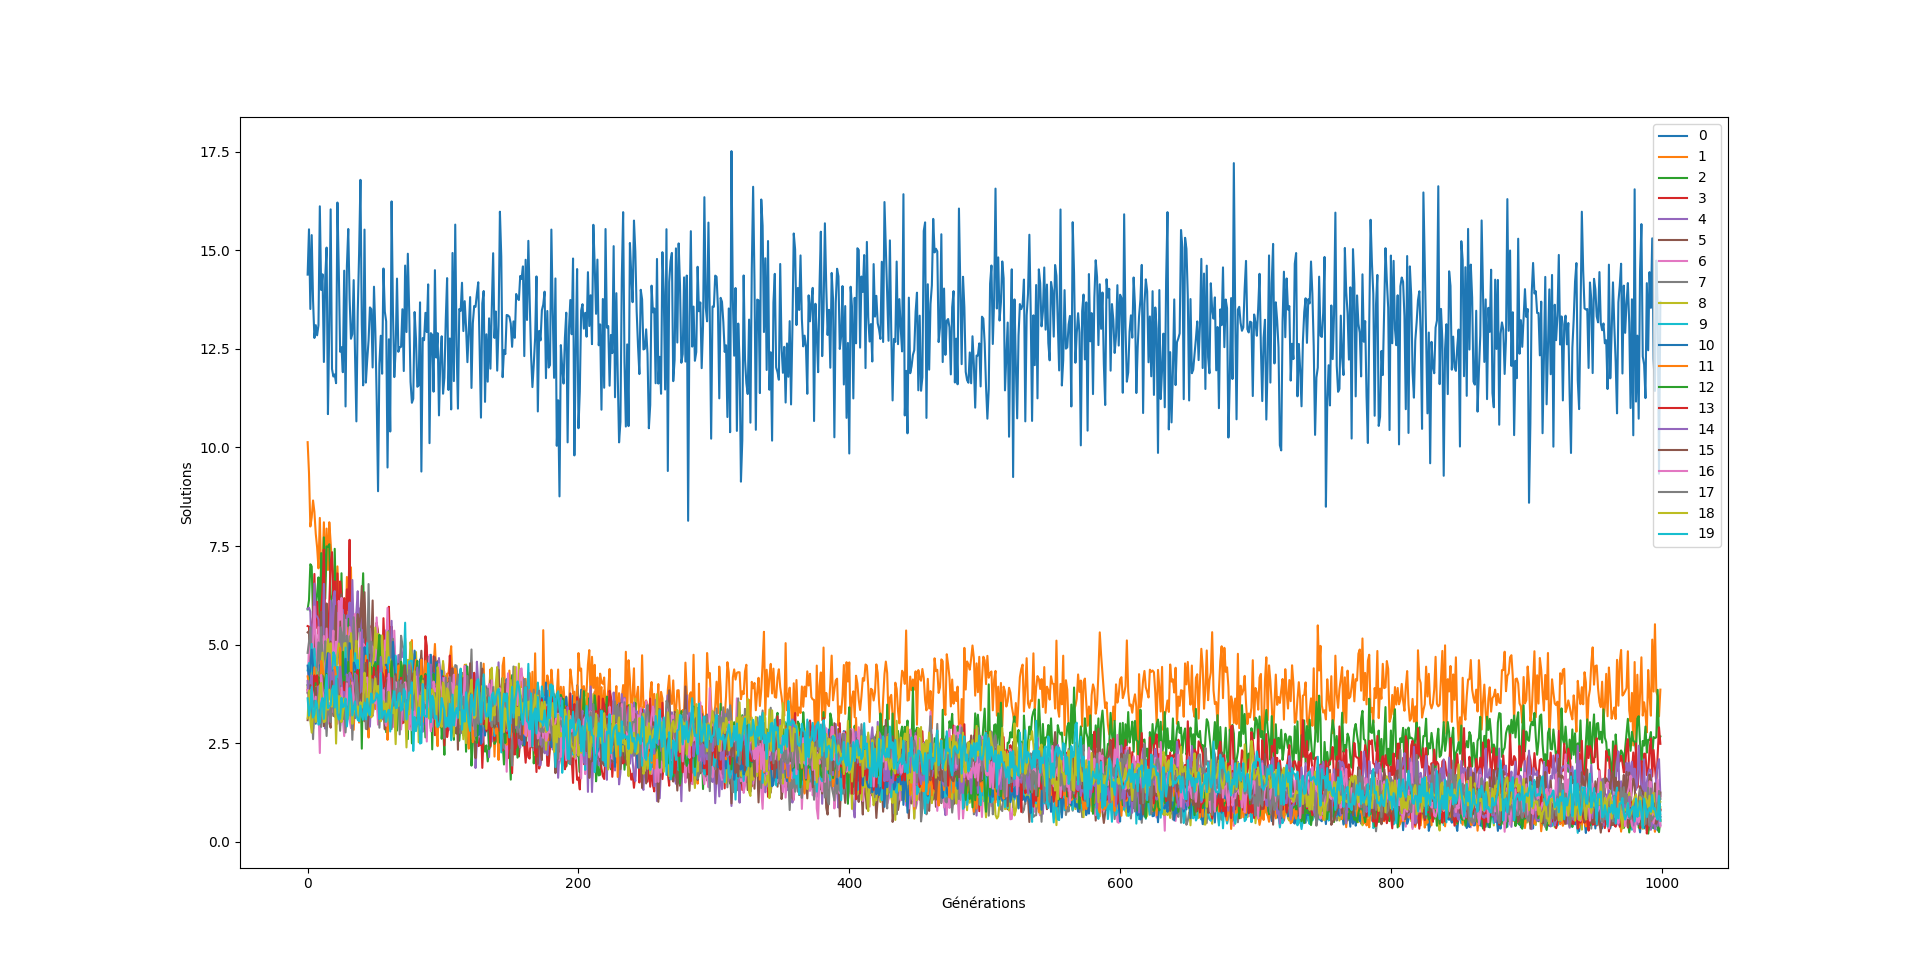
\includegraphics[width=18cm]{img/evo_pop_size_brut.png}
          \caption{Représentation de la solution au cours des générations - Variation de la taille de la population sur [10,2000] avec un pas de 10 - Autre paramètres : $P_{mutation} = 0.5$,$P_{crossover} = 0.5$}
          \label{evo_pop_size_brut}
        \end{figure}

        \begin{figure}[!]
          \centering
          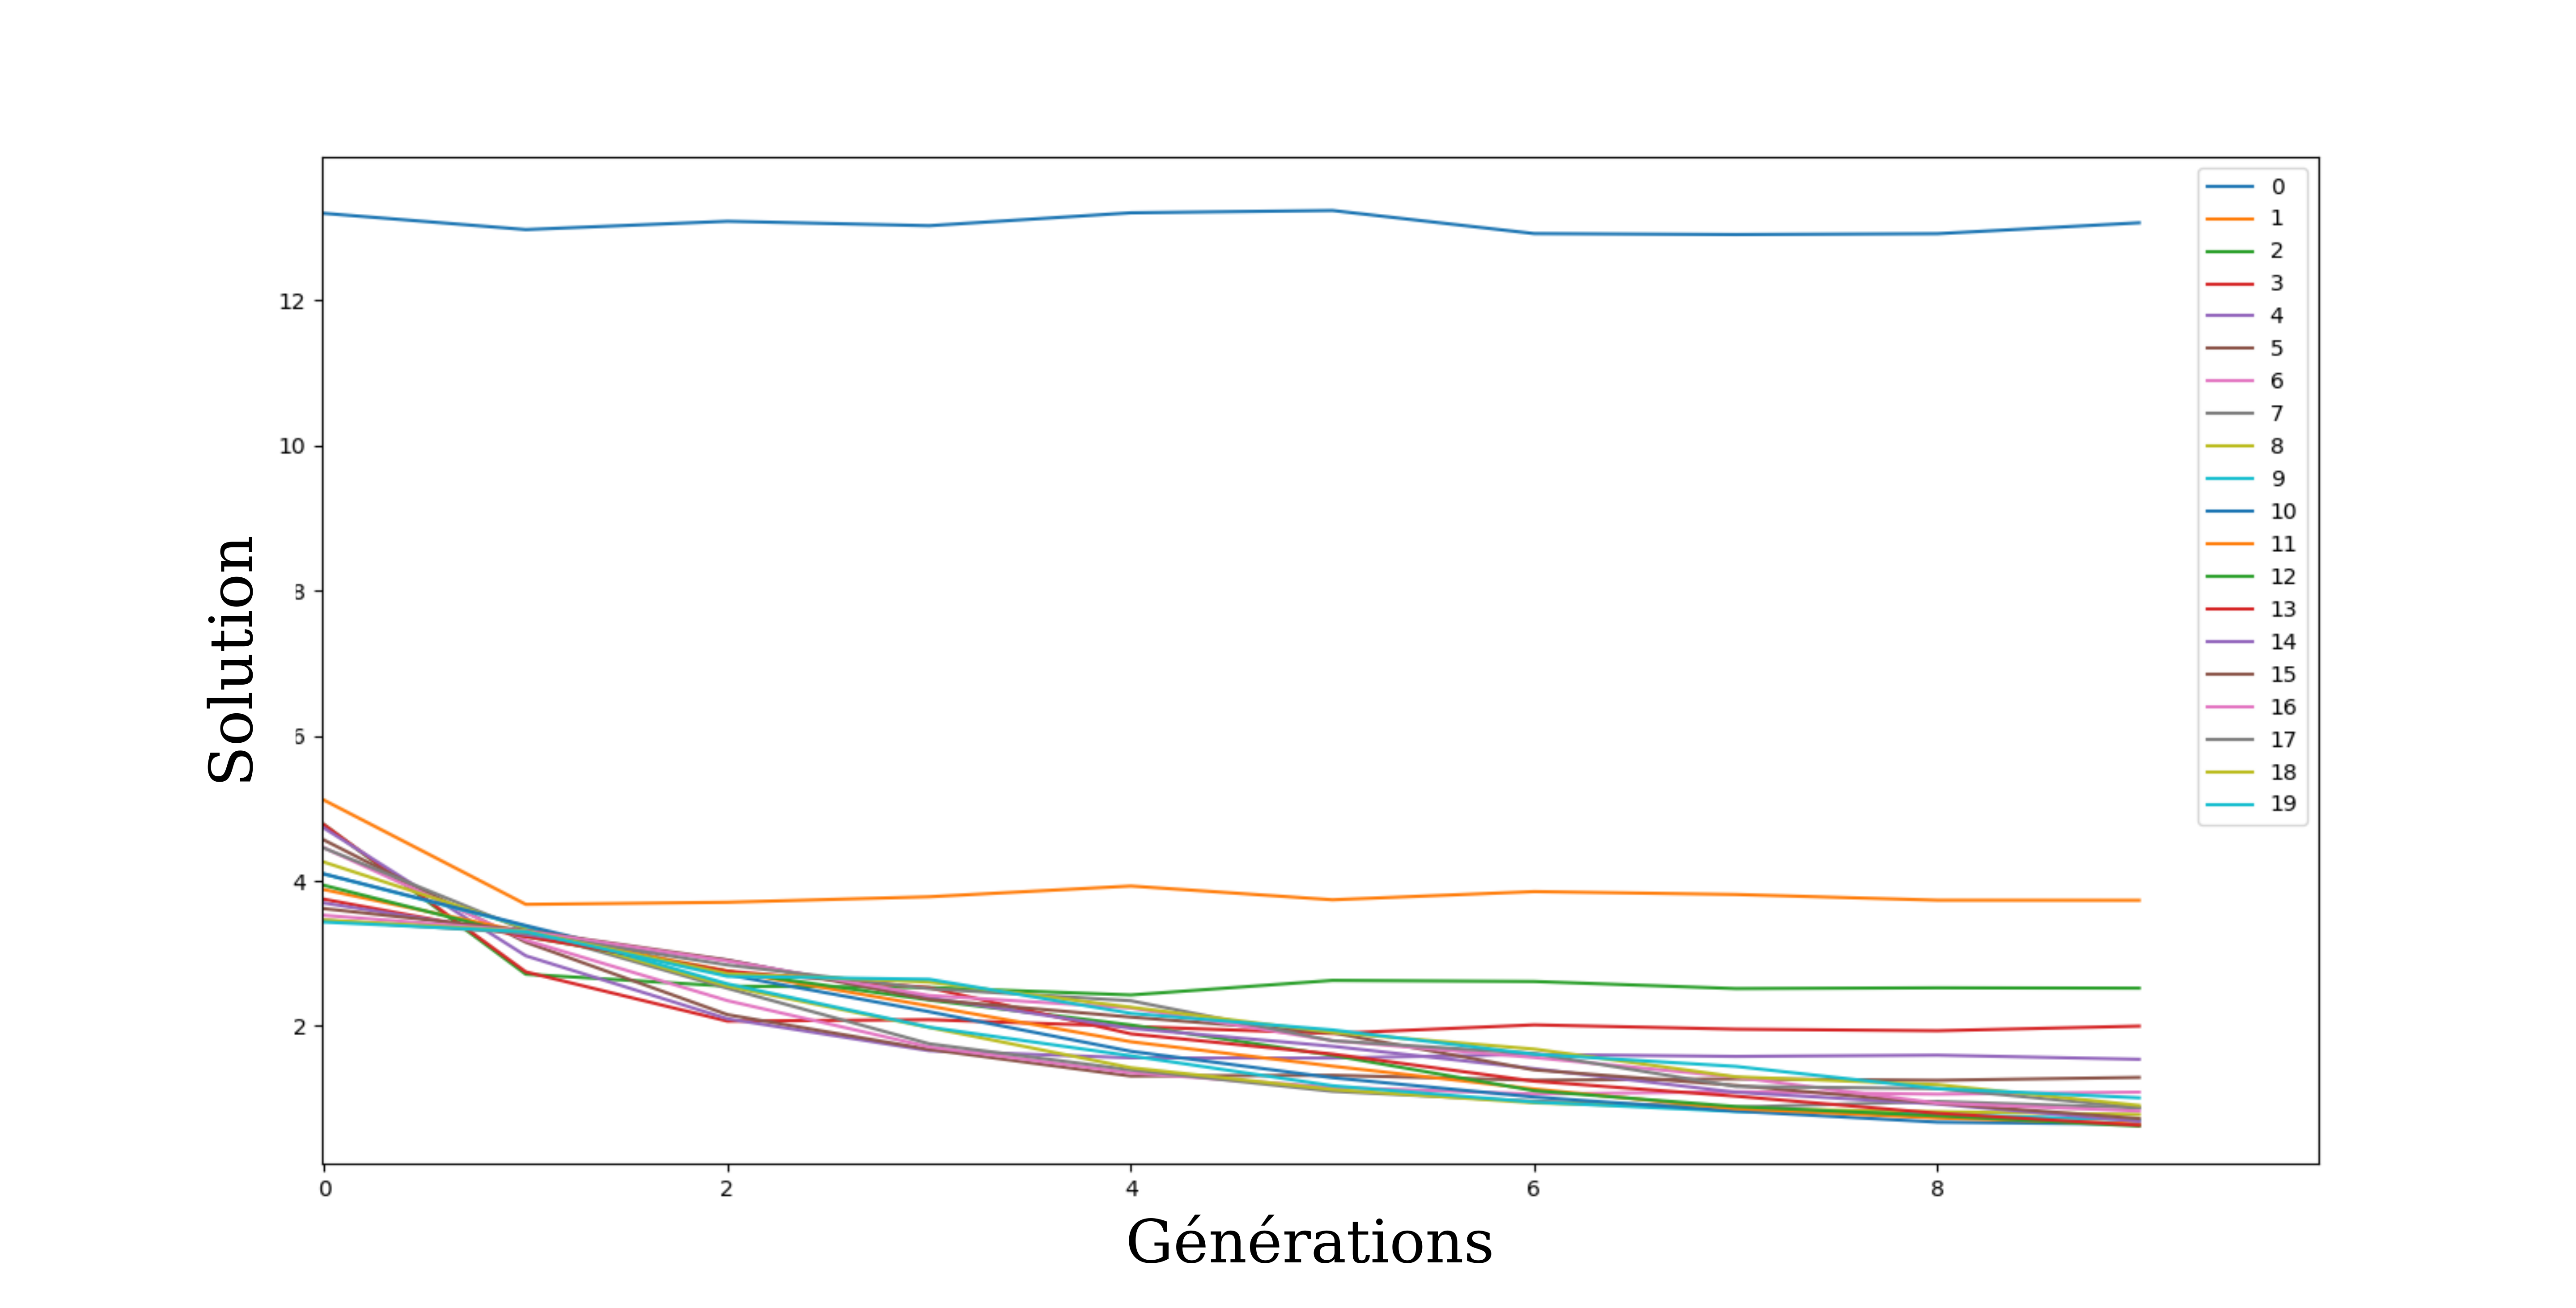
\includegraphics[width=18cm]{img/evo_pop_size_moy.png}
          \caption{Représentation "lissée" de la figure \ref{evo_pop_size_brut}}
          \label{evo_pop_size_moy}
        \end{figure}

        Le premier graphique (\ref{evo_pop_size_brut}) représente les données tel qu'elles sortent de notre algorithme, or bien que cette réprésentation soit précise et exacte, elle ne permet pas de tirer une conclusion quant à l'influence de ce paramètre. Afin d'éclaircir la figure on ramène un ensemble de points à une valeur moyenne de ces derniers, on obtient alors la figure \ref{evo_pop_size_moy}. \\

        Dans un premier temps on remarque que la première courbe qui a été générée est largement au dessus des autres. Cette courbe correspond à une taille de population de 10 alors que la suivante correspond à une population de 110. Dans les faits, quand la population est très faible (Moins de 100 individus) la convergence vers une solution de bonne qualité est très rapide, et donc n'est pas représentée de façon optimale sur ce graphique.

        Si on met cette première courbe de côté, on remarque dans un second temps que lors des premières générations la convergence est semblable pour toutes les courbes, mais que plus on avance dans les génération, plus les courbes s'écartent.



      \subsection{Probabilité de croisement}

      \begin{figure}[h]
        \centering
        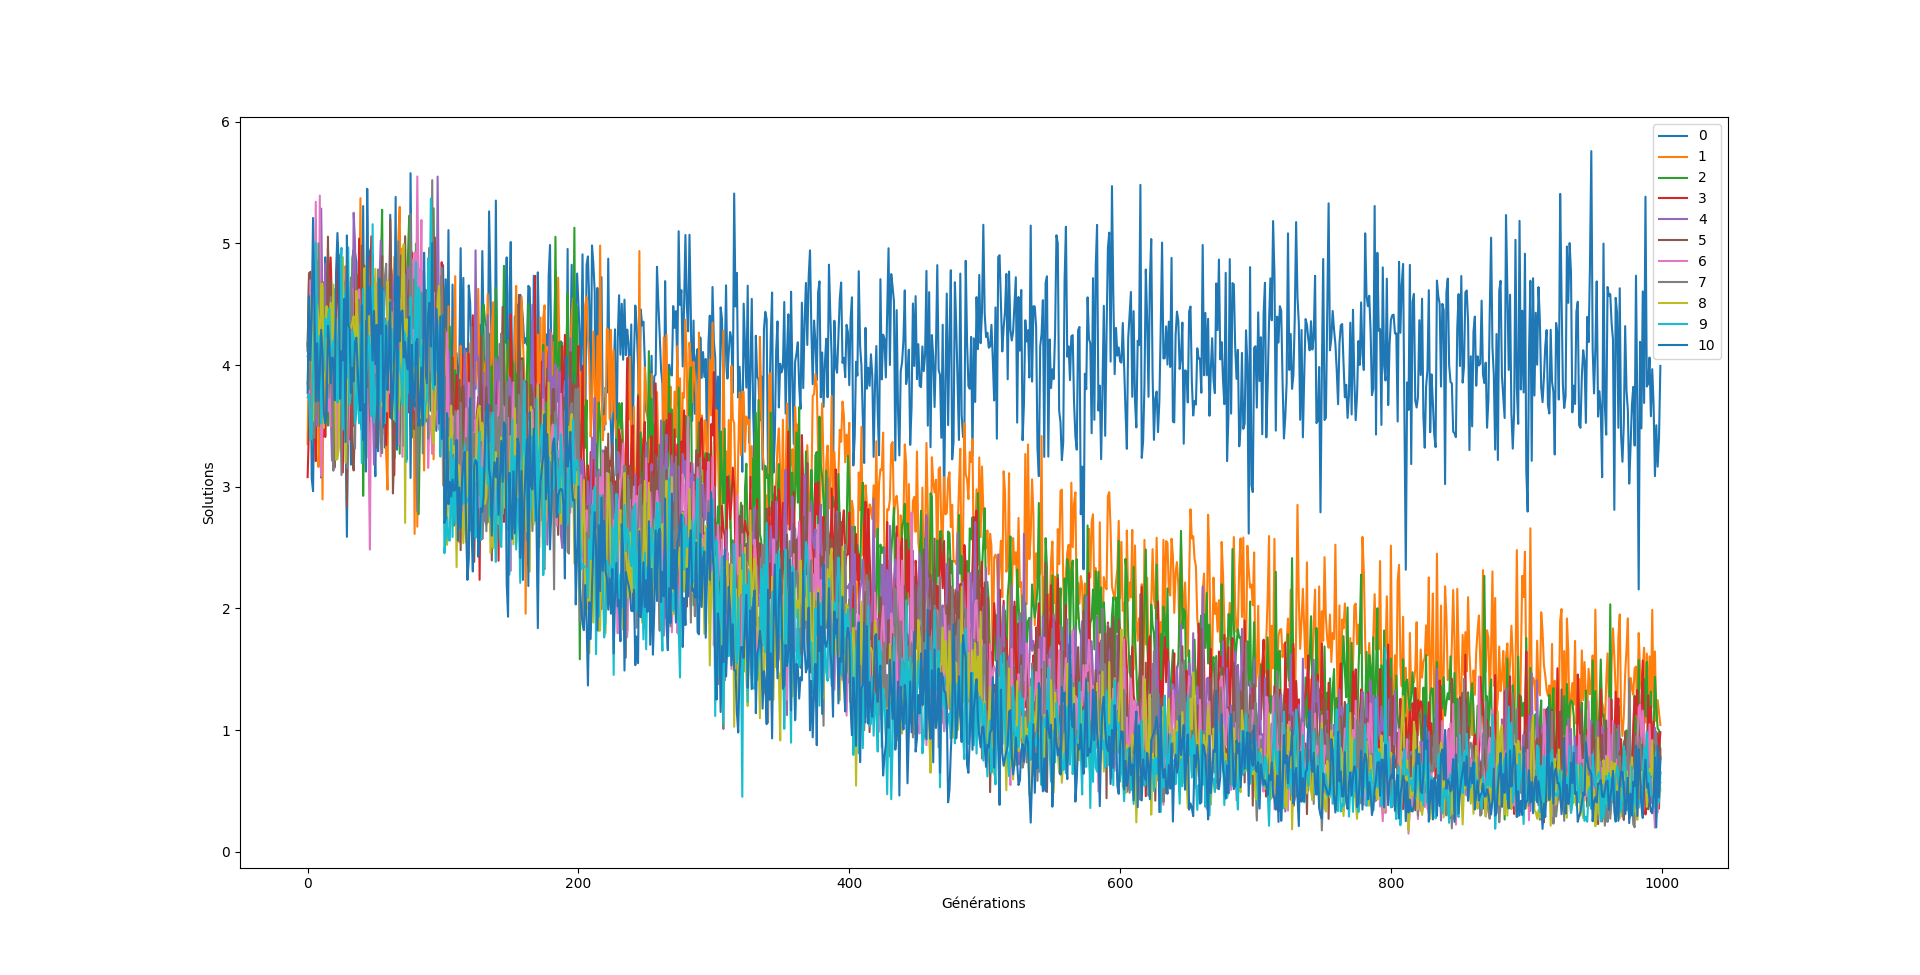
\includegraphics[width=15cm]{img/evo_crossover_brut.png}
        \caption{Représentation de la solution au cours des générations - Variation de la taille de la population sur [10,2000] avec un pas de 10 - Autre paramètres : $P_{mutation} = 0.5$,$population = 1000$}
        \label{evo_crossover_brut}
      \end{figure}

      \begin{figure}[!]
        \centering
        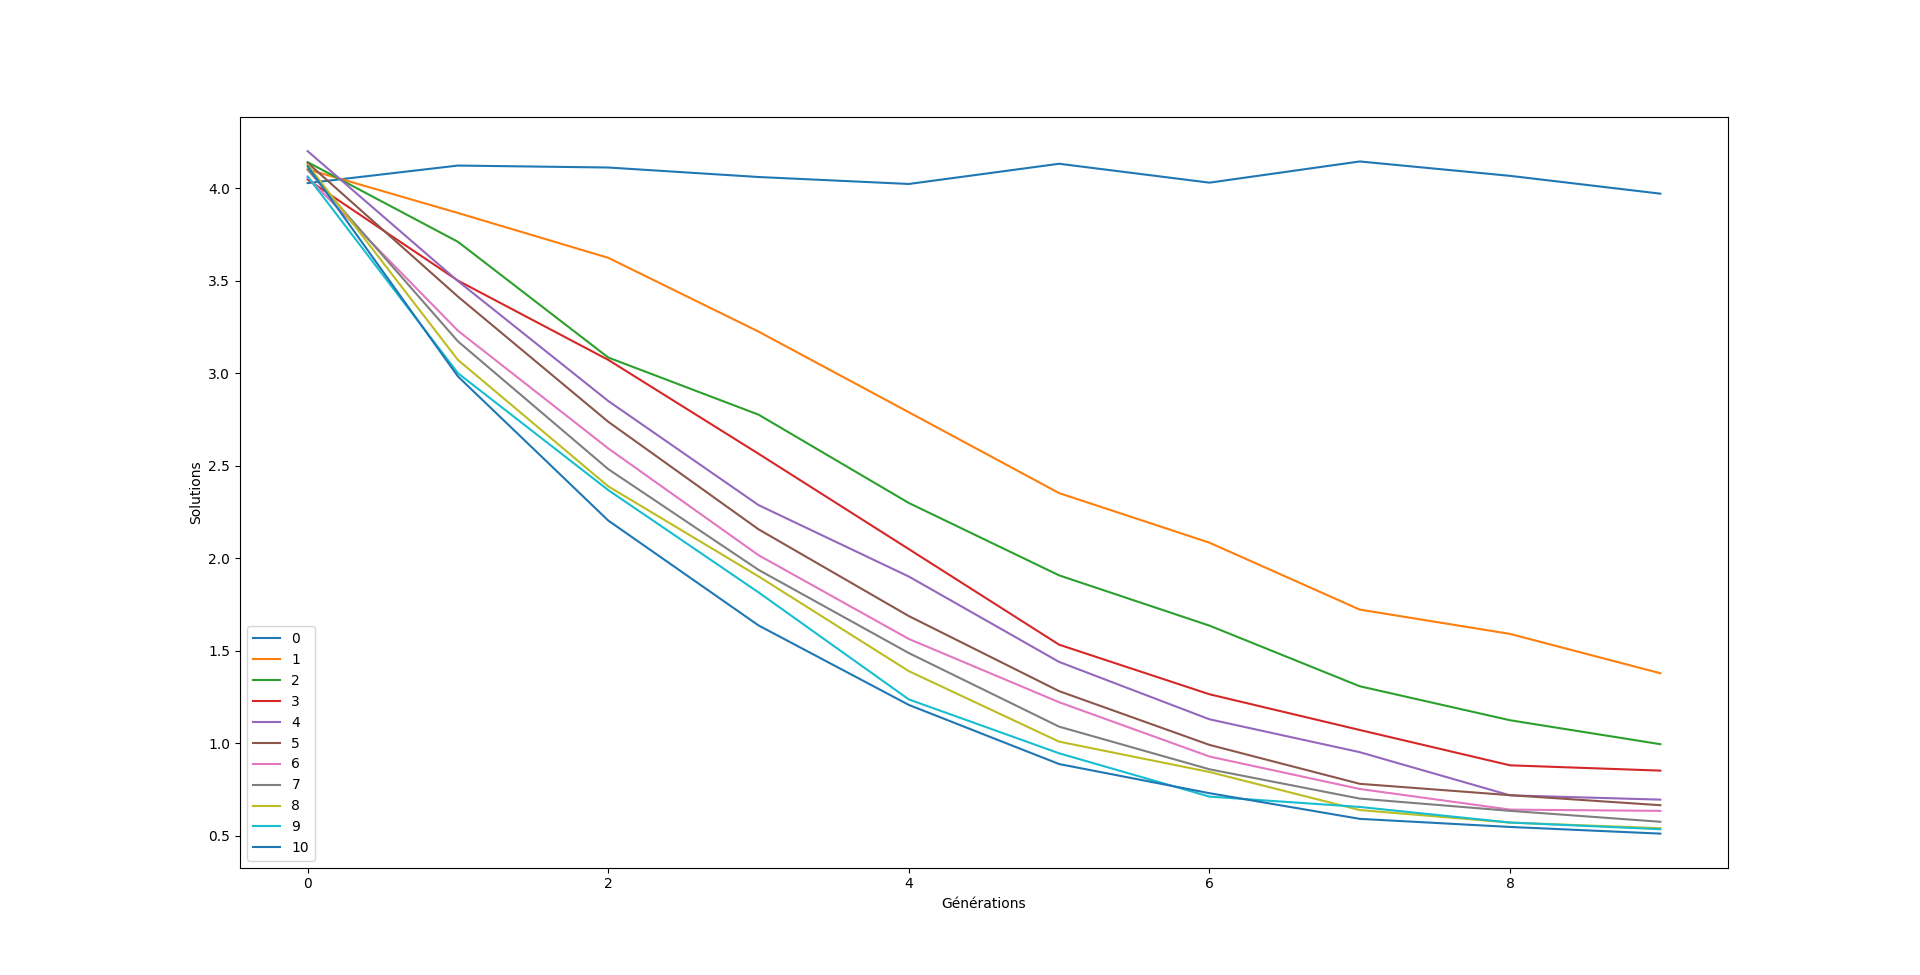
\includegraphics[width=15cm]{img/evo_crossover_moy.png}
        \caption{Représentation "lissée" de la figure \ref{evo_pop_size_brut}}
        \label{evo_crossover_moy}
      \end{figure}

      \subsection{Probabilité de mutation}

      \begin{figure}[h]
        \centering
        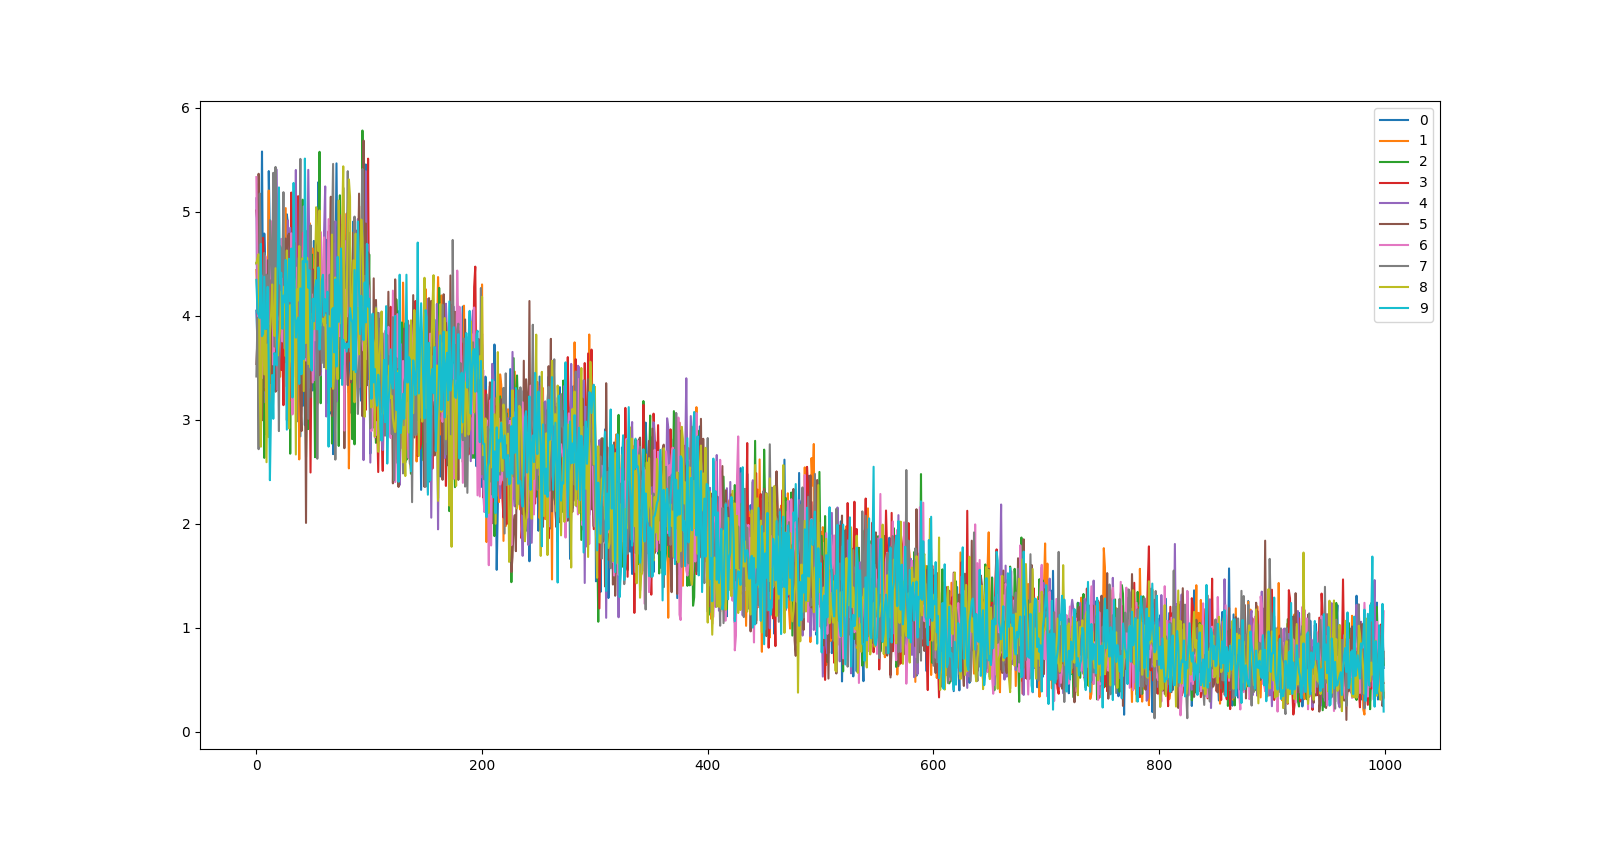
\includegraphics[width=15cm]{img/evo_mutation_brut.png}
        \caption{Représentation de la solution au cours des générations - Variation de la taille de la population sur [10,2000] avec un pas de 10 - Autre paramètres : $population = 1000$,$P_{crossover} = 0.5$}
        \label{evo_mutation_brut}
      \end{figure}

      \begin{figure}[!]
        \centering
        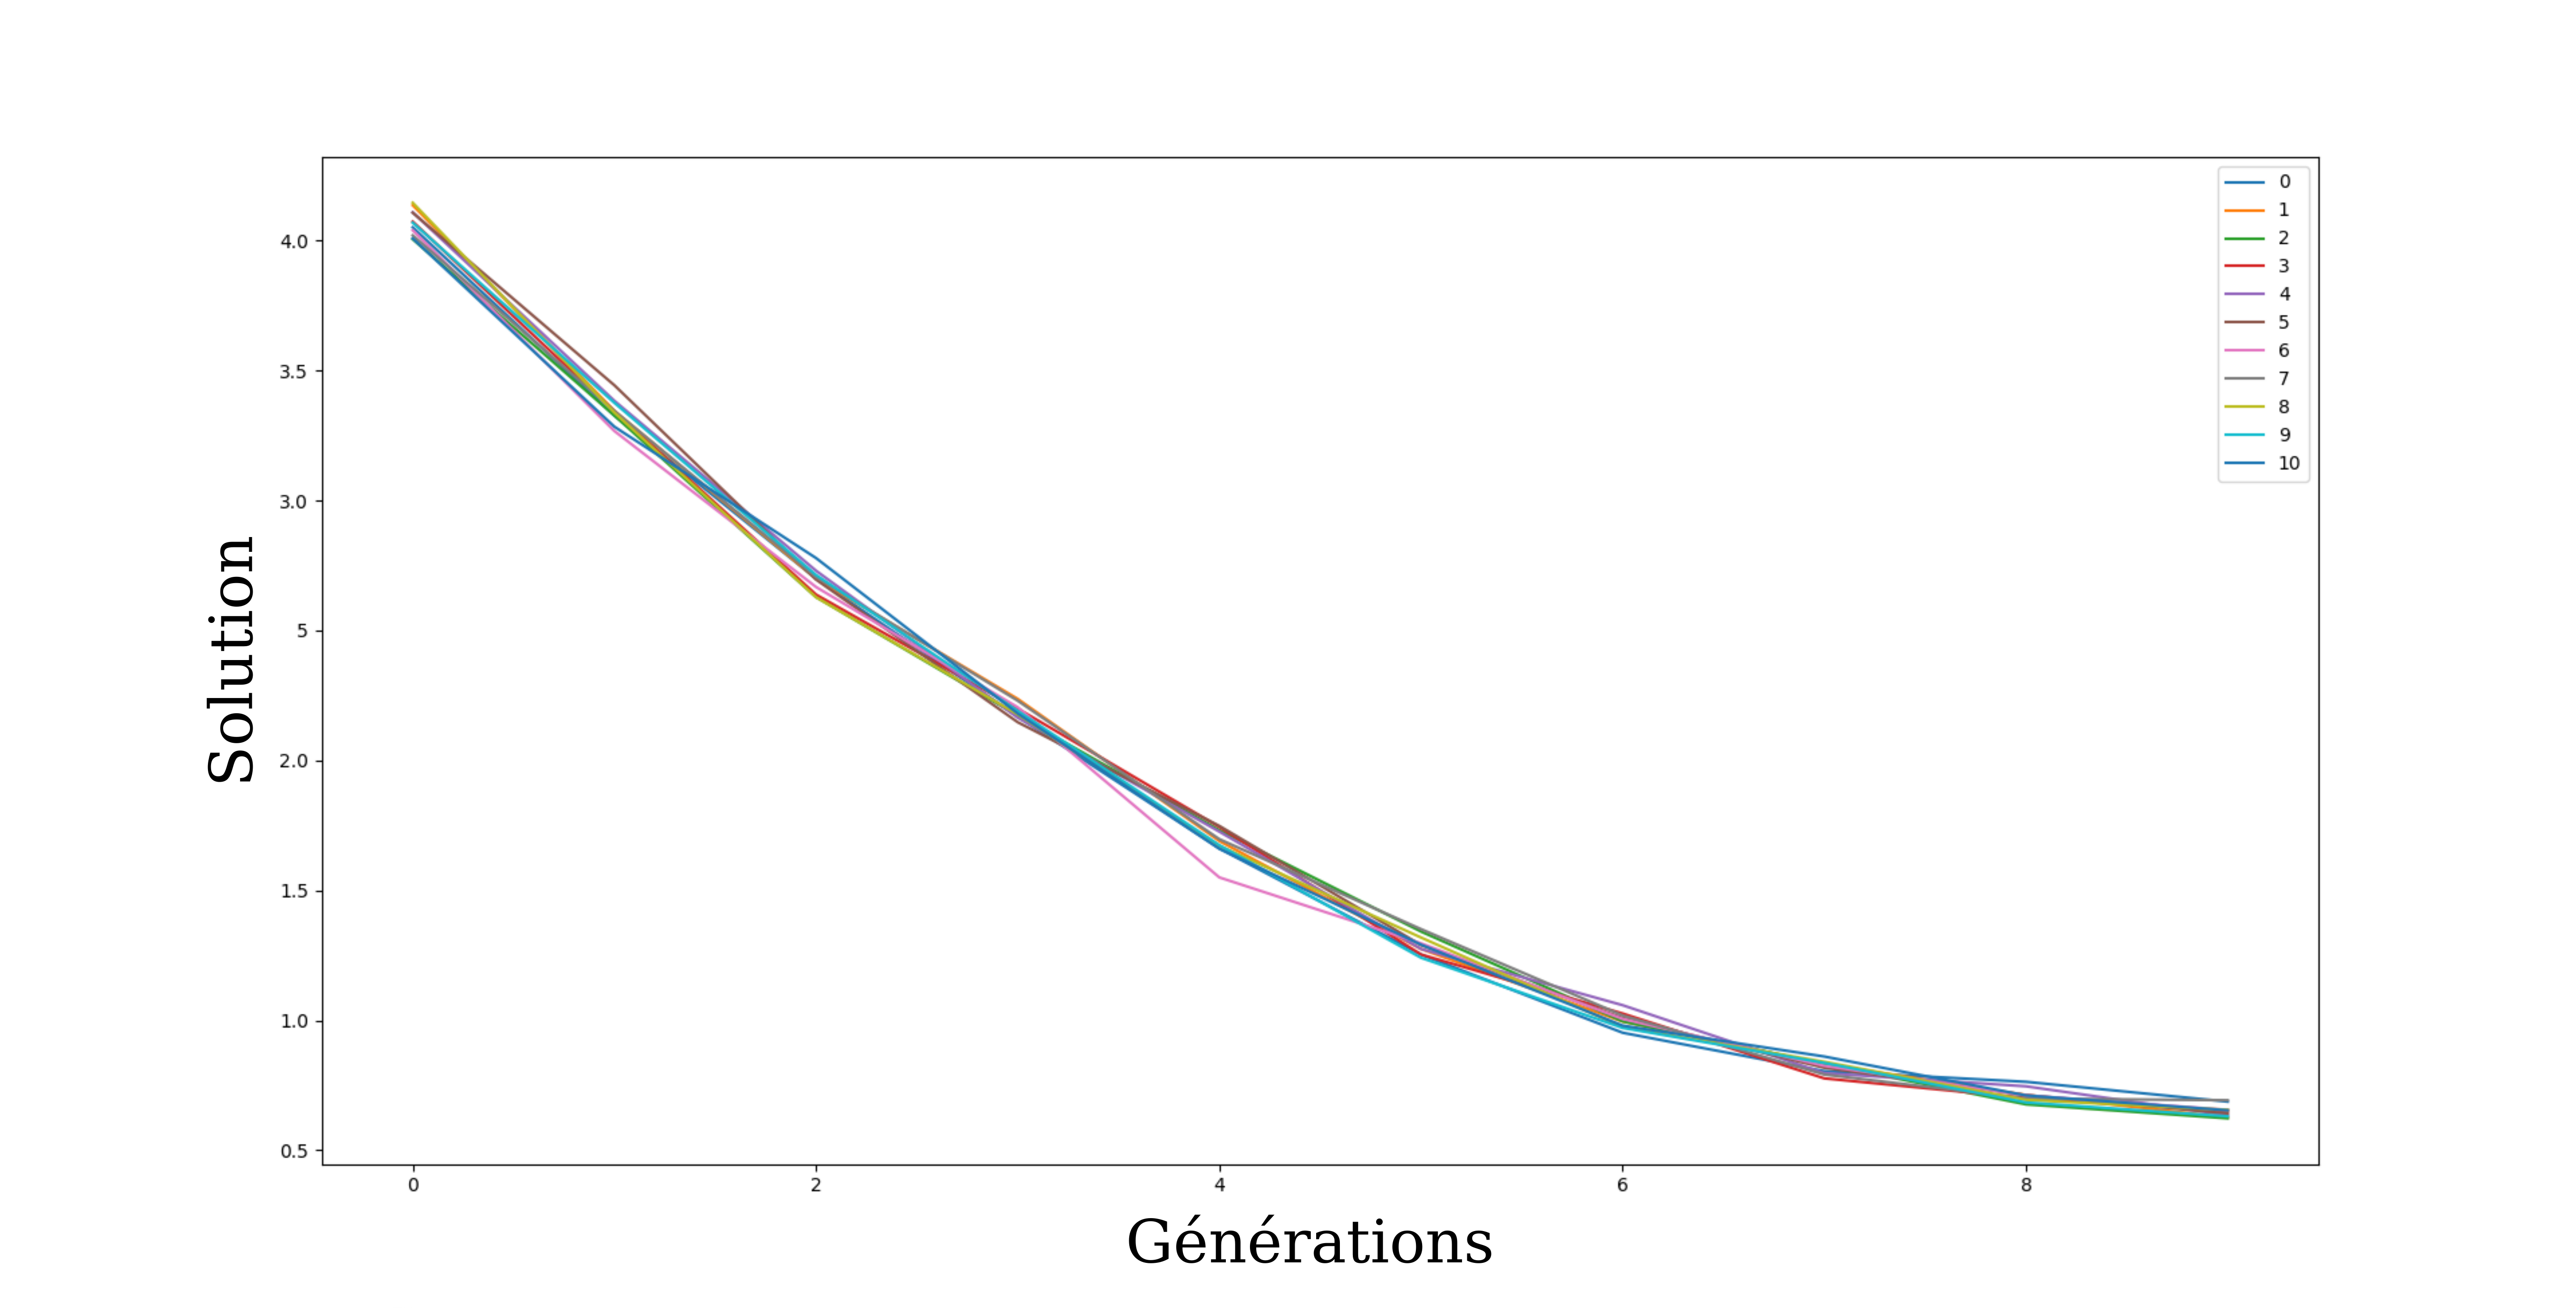
\includegraphics[width=15cm]{img/evo_mutation_moy.png}
        \caption{Représentation "lissée" de la figure \ref{evo_pop_size_brut}}
        \label{evo_mutation_moy}
      \end{figure}






  \chapter{Optimisation à objectifs multiples}
    \section{Algorithme - NSGAII}
    L'algorithmes d'optimisation NSGAII (Non dominated sorting genetic algorithm 2) est un algorithme connu et utilisé à l'échelle mondiale pour sa fiabilité et ses performances. Ce type d'algorithme diffère du premier par le nombre d'objectif qu'il peut prendre en paramètre. Quant bien le premier algorithme ne pouvait chercher une solution que sur un problème mono-objectif, l'algorithme NSGA-II peut prendre plusieurs objectifs en paramètre. Cette différence entraine le changement de la nature des solutions, on parle alors de \emph{front de Pareto. (Ou d'optimum de Pareto)}\\

    \begin{figure}[h]
      \begin{minipage}[c]{.46\linewidth}
          \centering
          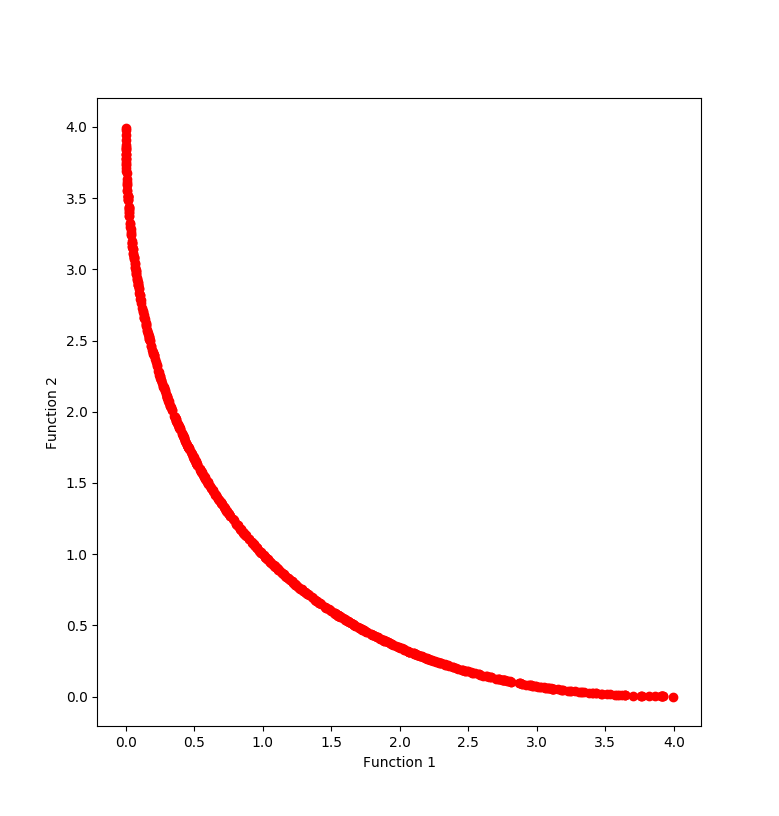
\includegraphics[width=6cm]{img/4,1,1_Pareto_uni.png}
          \caption{Front de Pareto du problème Schaffer N\degre1 \cite{wiki5} (bi-objectif)}
          \label{sch}
      \end{minipage}
      \hfill%
      \begin{minipage}[c]{.46\linewidth}
          \centering
          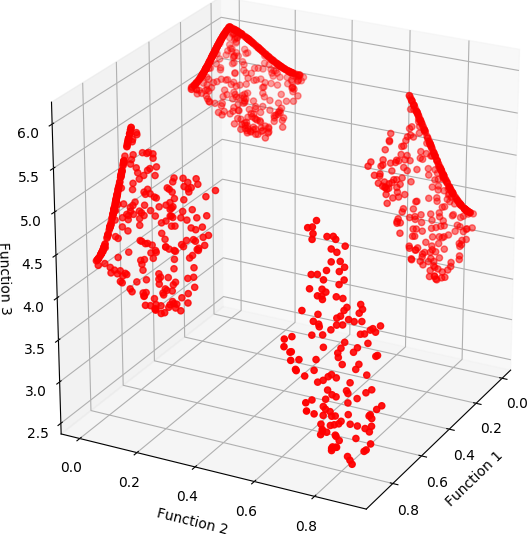
\includegraphics[width=6cm]{img/4,1,1_Pareto.png}
          \caption{Front de Pareto du problème DTLZ7 (tri-objectif)}
      \end{minipage}
    \end{figure}

    Le front de Pareto est une représentation graphique (figure \ref{sch}) de l'affirmation suivante :
    \begin{quotation}
      Il n'est pas possible d'ameliorer la qualité de solution d'un objectif sans faire baisser celles des autres.}.
    \end{quotation}

    \emph{Remarque : Le front de Pareto ne donne pas directement les solutions du problème, car il s'agit de la représentation des images des solutions. Le but ici est de choisir un point sur le front de Pareto et d'aller chercher ensuite son(es) antécédent(s) pour chaque objectif.}

    \begin{quotation}
      Exemple : Dans le cas d'un problème bi-objectif unidimentionel, pour un point $(a,b)$ sur le front de Pareto, la solution du problème est le doublet $(x,y)$ tel que $f(x)=a$ et $g(y)=b$.
    \end{quotation}

    Contrairement au premier algorithme qui ne retournait qu'une unique solution, la méthode NSGA-II offre un degré de liberté supplémentaire à son utilisteur. En effet, au vu de la multitude de point sur le front de Pareto, on peut se demander lequel retenir définitivement.
    \emph{A TERMINER}

      \subsection{Principe}
      \begin{wrapfigure}{r}{7cm}
        \centering
        \includegraphics[width=6cm]{img/Pareto_domine.png}
        \caption{Front de Pareto - individus dominés/non dominés}
        \label{non_domine}
      \end{wrapfigure}
      L'algorithme NSGA-II reprend le principe de l'algorithme présenté dans la première partie, mais comporte quelques caractéristiques supplémentaires.


      \begin{description}
        \item [Approche élitiste] L'algorithme sauvegarde les meilleurs solutions des générations précédentes (= préservation de la diversité)
        \item [Non domination] L'algorithme tri les individus selon un ordre croissant de non-domination (Voir figure \ref{non_domine})
        \item [Croisement linéaire] Contrairement au croisement à n points du premier algorithme, les portions caractéristiques de chaque individus sont échangées aléatoirement et non par segment.
        \item [Mutation personnalisé] L'algorithme propose de choisir la méthode de mutation à utiliser \cite{wiki6}. Dans notre cas, la mutation gaussienne est utilisé du fait de sa popularité après des utilisateurs de la bibliothèque Inspyred.
      \end{description}

      \begin{figure}[h]
        \centering
        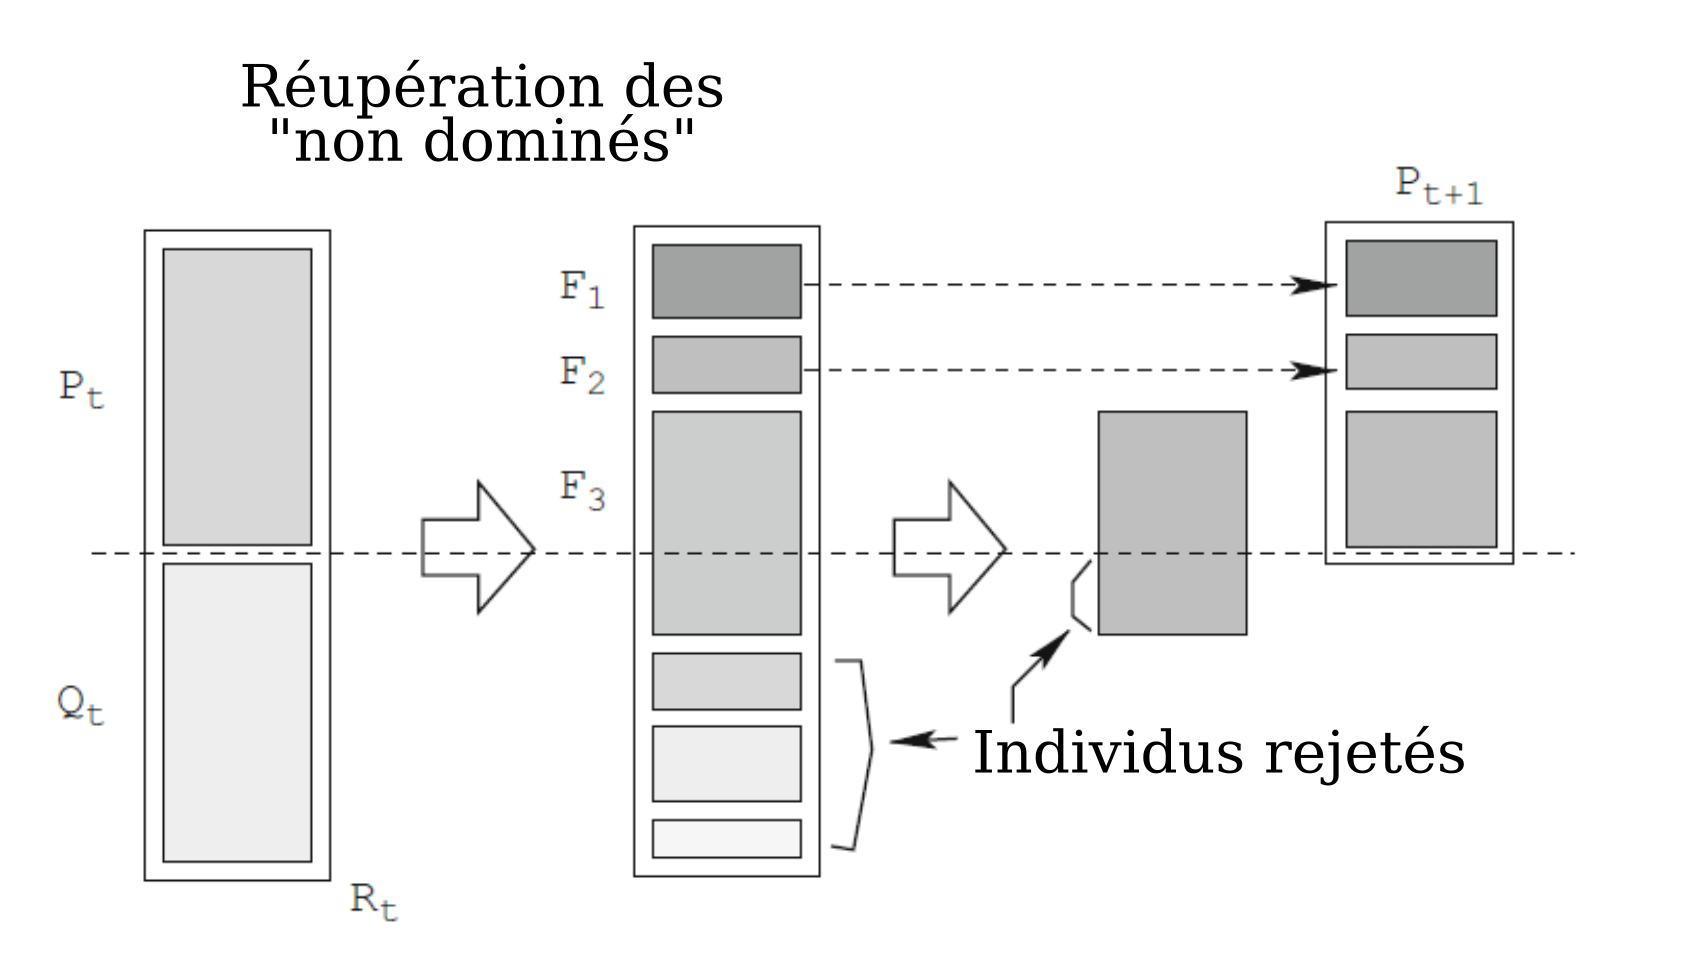
\includegraphics[width=12cm]{img/sch_nsga2.png}
        \caption{Schéma de fonctionnement NSGA2}
        \label{sch_nsga2}
      \end{figure}

      \emph{La figure \ref{sch_nsga2} schématise le fonctionnement de l'algorithme}
      \begin{enumerate}
        \item Initialement, une population d'individus est formée aléatoirement puis est triée sur le principe de non-domination.
        \item Les individus résulants forment la population $P_{t}$ (figure \ref{sch_nsga2}) qui se dédouble en $Q_{t}$ par croisement et mutation.
        \item L'ensemble $R_{t}$ est ensuite trié toujours sur le principe de non-domination, puis divisé en deux (En rejetant les individus à l'indice de domination trop élevé).
        \item On se retrouve alors avec une population $P_{t+1}$ prête à retourner à l'étape 2.
      \end{enumerate}


    \section{Méthode de comparaison des résultats}
      \begin{wrapfigure}{r}{5cm}
        \centering
        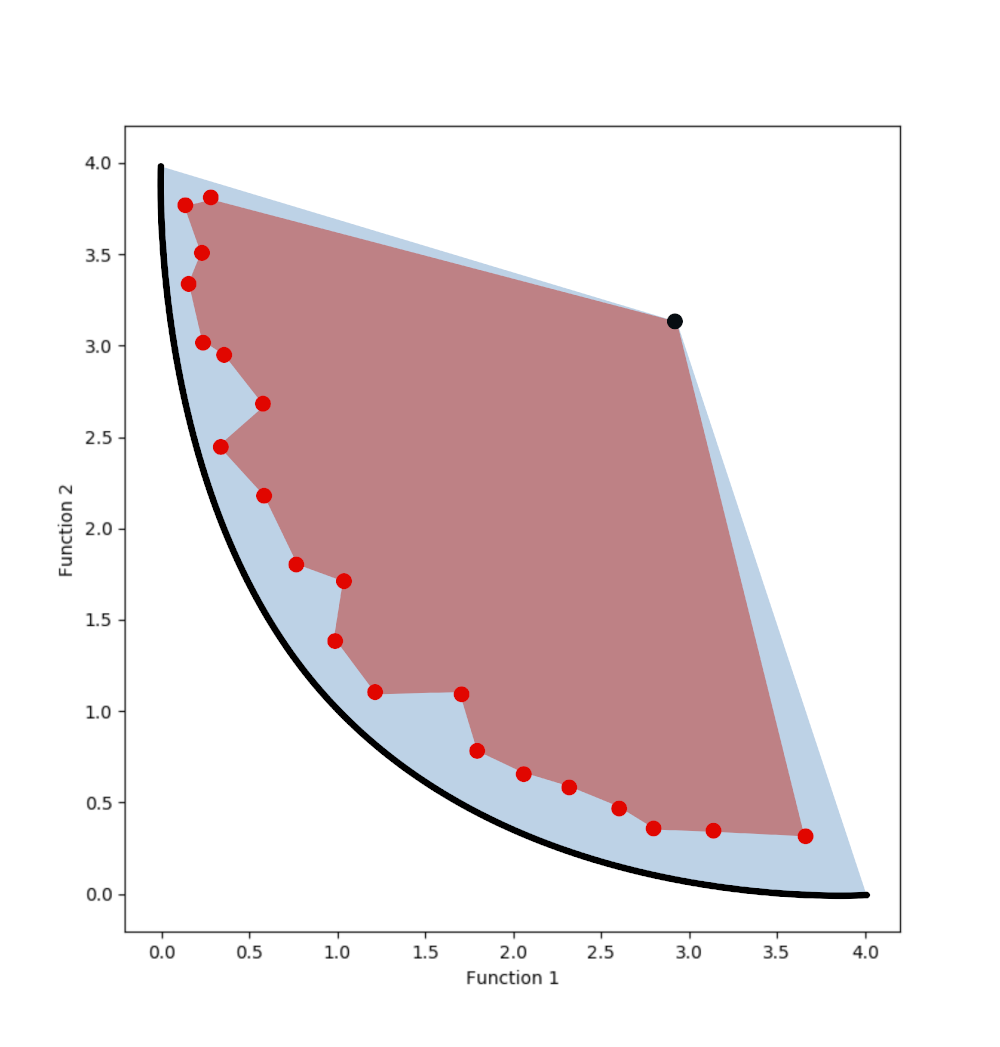
\includegraphics[width=6cm]{img/hypervolume.png}
        \caption{Représentation de la méthode de calcul du l'hypervolume}
        \label{hypervolume}
      \end{wrapfigure}
      Comme nous l'avons vu en abordant la notion de front de Pareto, le type solution recherché dans la cadre d'une optmisation multi-objectif n'est pas le même que dans un problème mono-objectif. Quant bien on cherchait une et une seule valeur avec le premier algorithme, l'objectif ici est de minimiser plusieurs fonction à la fois. Notre but final étant de d'étudier l'influence du paramétrage il est essentiel de pouvoir caractériser l'évolution de chaque algorithme. \\
      Dans le cas présent, pour un problème multi-objectif il est possible d'étudier l'évolution du front de Pareto géométriquement en calculant l'air, le volume ou plue généralement l'hypervolume de ce dernier.
      Prenons un exemple simple dans un problème ou l'on cherche à minimiser deux fonctions (Figure \ref{hypervolume}). La courbe noir représente le front de Pareto de référence et les points rouges un front trouvé à l'aide de l'algorithme NSGAII (Peu d'individus et peu de générations). On pose un point sur le plan et on calcule les aires des front noir et rouge en tenant compte du point A. On obtient alors deux valeurs réelles comparables qui permettent d'étudier la convergence du front de Pareto au cours des générations (Plus les valeurs sont semblables, plus la qualité du Pareto est bonne).
    \section{Influence du paramétrage}
      De la même façon qu'avec le premier algorithme on cherche à observer l'influence du paramétrage sur le qualité de la solution. La seul différence notable avec la première observation est que dans cette partie elle est basée sur l'évolution de l'hypervolume et non plus de la solution directement.
      \subsection{Taille de la population}
      \subsection{Probabilité de croisement}
      \subsection{Probabilité de mutation}


    \section{NSGA III}


  \chapter{Conclusion}
   + Il existe d'autre algo utilisés : http://www.laas.fr/files/MOGISA/sem_Alain-Berro.pdf p.31
   + Il faut relier avec le metier ingé

  \appendix

  \nocite{*} %On affiche toute la Bibliographie
  \bibliographystyle{plain}
  \bibliography{biblio}

  \chapter{Annexes}
    \subsection{Programme}
      \paragraph{}
      L'ensemble des programmes qui ont été utilisé pour réaliser ce projet sont mis à disposition sur notre page GitHub : \\\\
      \url{https://github.com/Akashita/AG-USMB}

      \paragraph{}
      Ce travail est soumis à la license \emph{GNU General Public License v3.0}\\ %\emph dit à latex que cette partie est importante
      Pour plus de détails veuillez vous référer au site gnu.org : \\\\
      \url{https://www.gnu.org/licenses/gpl-3.0.en.html}

    \subsection{Figures}






\end{document}
